\documentclass[11pt,a4paper,english,twoside,notitlepage,openright]{article}
%\usepackage{../thesis-iipr}

%\usepackage{caption}
\usepackage{subcaption}

% For tikz
\usepackage{pgf}
\usepackage{tikz}
\usetikzlibrary{arrows,automata,matrix,positioning,shapes,shapes.geometric}
%\usepackage{xcolor}

\usepackage{multirow}
\usepackage{makecell}

\begin{document}

\title{Recurring \LaTeX\, commands}
\author{Ignacio-Iker Prado-Rujas}
\date{\today}

\maketitle

\abstract{This document intends to gather common \LaTeX \,commands or functionalities that I tend to forget too fast.}

\tableofcontents
\newpage

\section{Including one or more images}

Simple single figure:
\begin{figure}[!h]
\centering
\includegraphics[scale=0.2]{figures/sin.png}
\caption{A nice figure.}
\label{fig:lab}
\end{figure}

Several figures as a table with a single caption:
\begin{figure*}[!h]
  \centering
  \begin{tabular}{cc}
    \includegraphics[scale=0.2]{figures/sin.png}
    &
    \includegraphics[scale=0.2]{figures/sin.png}
  \end{tabular}
  \caption{Another nice figure.}\label{fig:lab}
\end{figure*}

To use subfigures and subcaption, need to \verb|\usepackage{subcaption}|:
\begin{figure*}[!h]
     \centering
     \begin{subfigure}[b]{0.3\textwidth}
         \centering
         \includegraphics[width=\textwidth]{figures/sin.png}
         \caption{Caption 1.}
         \label{fig:lab}
     \end{subfigure}
     \hfill
     \begin{subfigure}[b]{0.3\textwidth}
         \centering
         \includegraphics[width=\textwidth]{figures/sin.png}
         \caption{Caption 2.}
         \label{fig:lab}
     \end{subfigure}
     \hfill
     \begin{subfigure}[b]{0.3\textwidth}
         \centering
         \includegraphics[width=\textwidth]{figures/sin.png}
         \caption{Caption 3.}
         \label{fig:lab}
     \end{subfigure}
        \caption{Three simple graphs}
        \label{fig:lab}
\end{figure*}



\section{Simple TikZ diagram}

\begin{verbatim}
\usepackage{pgf}
\usepackage{tikz}
\usetikzlibrary{arrows,automata,matrix,positioning,shapes,shapes.geometric}
%\usepackage{xcolor}
\end{verbatim}

\begin{center}
		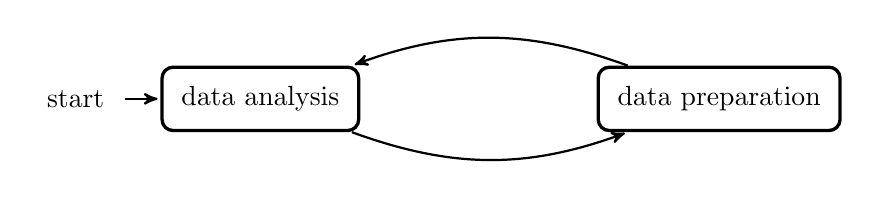
\begin{tikzpicture}[->,>= stealth',shorten >=1pt, auto, node distance=0.2cm, thick, inner sep=7pt, draw=black]
			\tikzset{rect/.style={rounded corners,very thick,draw=black,text=black}}
			% Colors: black, blue, darkGreen, red...
			
			% States
			\node[rect, initial] (q0) {data analysis};
			\node[rect] (q1) [right=3cm of q0] {data preparation};
			%Transitions in=180, out=220, bend angle=0
			\path 
				(q0)	edge [in=200,out=340]	node [align=center]		{ }	(q1)
				(q1)	edge [in=20,out=160]	node [align=center]		{ }	(q0)
				;
	\end{tikzpicture}
\end{center}

\section{Moving a table into the margin}

\begin{table*}[!h]
\caption{Original table position.}
\label{tab:lab}
\begin{center}
%\rotatebox{90}{ % If you want to rotate the table
\begin{tabular}{p{2cm}|p{2cm}|p{5cm}|p{5cm}}
\textbf{What?}    &    \textbf{Why?}    &    \textbf{How?}     &    \textbf{Where?}\\ \hline
This.             & That.               &    This other thing. & That other thing that is long. \\
That.             & This.               &    That other thing that is long. & This other thing. \\
\end{tabular}
%}
\end{center}
\end{table*}

Reference extent of text (\verb|\hrule|): \vspace{0.1cm}
\hrule
\begin{table*}[!h]
\caption{A nicer table.}
\label{tab:lab}
\begin{center}
\hspace*{-1.3cm}
%\rotatebox{90}{ % If you want to rotate the table
\begin{tabular}{p{2cm}|p{2cm}|p{5cm}|p{5cm}}
\textbf{What?}    &    \textbf{Why?}    &    \textbf{How?}     &    \textbf{Where?}\\ \hline
This.             & That.               &    This other thing. & That other thing that is long. \\
That.             & This.               &    That other thing that is long. & This other thing. \\
\end{tabular}
%}
\end{center}
\end{table*}

\section{Multirows and multicolumns}

\begin{verbatim}
\usepackage{multirow}
\usepackage{makecell}
\end{verbatim}

\begin{table*}[!h]
\caption{A cool table.}
\label{tab:lab}
\begin{center}
%\rotatebox{90}{ % If you want to rotate the table
\begin{tabular}{m{2cm}||m{2cm}|m{3cm}|m{3cm}}
\multirow{2}{*}{\textbf{What?}} & \multicolumn{3}{c}{\textbf{Context}} \\ \cline{2-4}
& {Why?}    &    {How?}     &    {Where?}\\ \hline\hline
                                            & That. & This other thing. & That other thing. \\
\multirow{2}{*}{\makecell{Common \\ thing}} & That. & This other thing. & That other thing. \\
                                            & This. & That other thing. & This other thing. \\
                                            & That. & This other thing. & That other thing. \\
\end{tabular}
%}
\end{center}
\end{table*}

\end{document}